We're going to use a word a lot in this book: \emph{learned}. Before we
do, we have to be honest about what it means --- because ``the model
learned to add'' is a sentence people say all the time, and it's usually
hiding a big assumption.

\section{A simple way to think about
it}\label{a-simple-way-to-think-about-it}

Imagine a child who aces a worksheet of addition problems. Every problem
is like ``4 + 3 = ?'' and the child gets them all right. We'd be tempted
to say ``the child can add.''

But there are two very different ways to get that perfect score:

\begin{enumerate}
\def\labelenumi{\arabic{enumi}.}
\tightlist
\item
  The child \emph{understands addition} --- show them ``37 + 58'' and
  they solve it, because they know how to add any two numbers.
\item
  The child \emph{memorized the exact answers} --- they've seen these
  exact problems before and just remember that ``4 + 3 = 7,'' but hand
  them a problem they've never seen and they freeze.
\end{enumerate}

A perfect worksheet grade can't tell these two apart. \textbf{The
worksheet is a bad test.} Only a \emph{new} problem can.

This is the entire premise of the book in one image. Our model gets a
perfect-ish worksheet sometimes. The question is always: would it pass
the \emph{new} problem?

\section{What ``learned'' means here}\label{what-learned-means-here}

So we define it narrowly and honestly. A model shows \textbf{learned
capability} when, to the degree the evidence supports:

\begin{enumerate}
\def\labelenumi{\arabic{enumi}.}
\tightlist
\item
  \textbf{It gets better as it trains} --- the loss falls, and the thing
  we care about reliably improves.
\item
  \textbf{It works on examples it never saw} --- not just the ones in
  training.
\item
  \textbf{It survives harmless changes} --- different variable names,
  different wording, a different way of saying the same instruction.
\item
  \textbf{It can combine things it knows} --- put two learned pieces
  together in a new arrangement, not just repeat an arrangement it
  already saw.
\item
  \textbf{Simpler explanations have been ruled out.} The mundane
  alternatives --- memorization, copying a near-duplicate, a template, a
  leaked test, a buggy evaluator --- must be tested and rejected.
\end{enumerate}

We are deliberately \textbf{not} asking whether the model ``really
understands'' in a philosophical sense. We're asking narrower,
answerable things: does it generalize? to what? and could a dumber
mechanism explain the result?

\section{The four levels of
generalization}\label{the-four-levels-of-generalization}

\begin{figure}
\centering
\pandocbounded{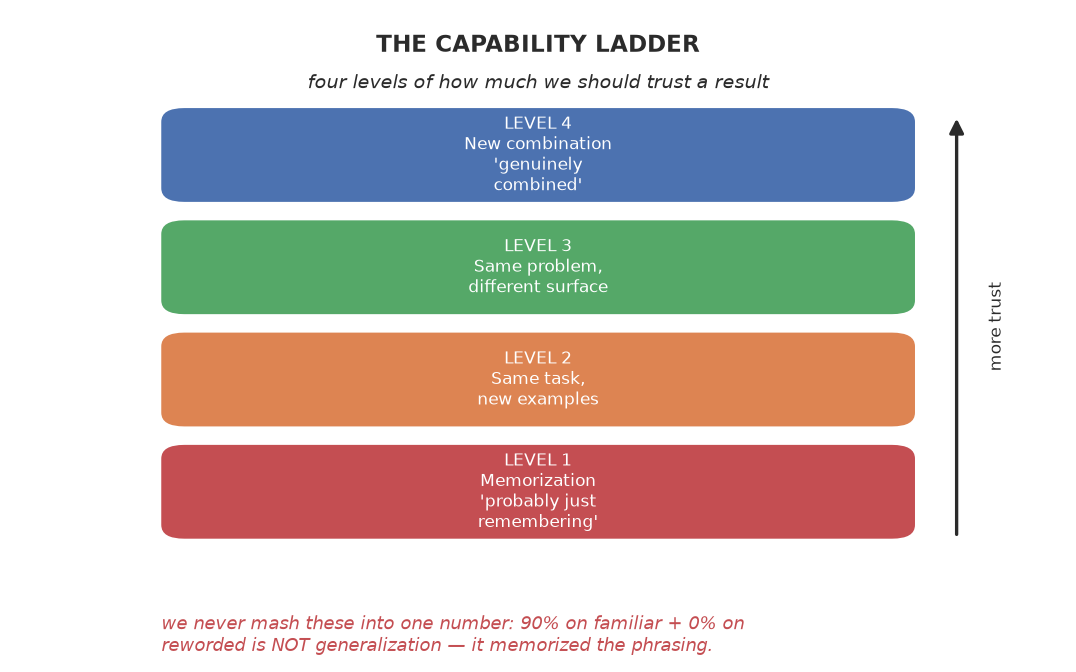
\includegraphics[keepaspectratio,alt={The capability ladder},width=\maxwidth{\textwidth},keepaspectratio]{figures/fig_ladder.png}}
\caption{The capability ladder}
\end{figure}

The ladder makes the four questions explicit. Each rung asks us to trust
a result a little more; we never collapse them into a single number.

This is the book's organizing idea. It is a ladder of how much we should
trust a result --- from ``probably just remembered'' to ``genuinely
combined.''

\textbf{Level 1 --- Memorization.} The model reproduces something it saw
in training: an exact example, an exact constant, a familiar phrase, a
near-duplicate. \emph{Question: could this just be remembering?}

\textbf{Level 2 --- Same task, new examples.} The model works on a new
instance of the same kind of problem. \emph{Question: does it work on
problems it hasn't seen before?}

\textbf{Level 3 --- Same problem, different surface.} The computation is
identical, but the \emph{outer layer} changes: new numbers, new variable
names, reworded instruction, harmless distractors. \emph{Question: does
it survive changes that shouldn't matter?}

\textbf{Level 4 --- New combination.} The model must combine pieces it
knows into something that never appeared in training. It learned A, B,
and C separately --- can it do A \emph{sandwiched inside} B, or A
followed by C? \emph{Question: can it put things together, or only
repeat what it already saw?}

\textbf{A rule we'll follow strictly:} never mash these four into one
number. A model that scores 90\% on familiar problems and 0\% on a
reworded version has not ``generalized'' --- it memorized the phrasing.
One number would hide exactly the thing we care about.

\section{The recurring question: ``how did it
cheat?''}\label{the-recurring-question-how-did-it-cheat}

Because we refuse to trust a single score, every experiment asks the
same skeptical question:

\begin{quote}
\textbf{How could the model have gotten this without learning what we
think it learned?}
\end{quote}

The usual suspects are always on the table: memorized templates,
memorized constants, memorized name patterns, wording quirks, unbalanced
data, train/test leakage, near-duplicates, retrieval, a weak evaluator,
hardcoded answers, hidden-test leakage.

Every major experiment therefore ends with a \textbf{shortcut audit},
six steps: (1) the suspected cheat, (2) why it could explain the result,
(3) a control test, (4) what the control found, (5) what that rules out,
and (6) what's still unresolved.

That audit --- not the headline number --- is the book's signature. It's
the difference between ``the model works'' and ``we know why the model
works.''
